\documentclass[acmsmall]{acmart}
\usepackage{hyperref}
\usepackage{hyperxmp}
\setcopyright{none}
\copyrightyear{2023}
\acmYear{2023}
\acmDOI{}

\citestyle{acmauthoryear}

\usepackage{hyperref}
\usepackage{hyperxmp}
\usepackage{fancyhdr}
\usepackage{fancyvrb}
\usepackage{algpseudocode}
\usepackage{algorithm}
\usepackage{graphicx}
\usepackage{wrapfig}
\begin{document}

\title{Synthesizing Recursive Programs Using Generic Folds}

\author{Rafaello Sanna}
\affiliation{%
  \institution{Harvard University}
  \country{USA}
}
\author{Nada Amin}
\affiliation{%
  \institution{Harvard University}
  \country{USA}
}
\author{William Byrd}
\affiliation{%
  \institution{University of Alabama at Birmingham}
  \country{USA}
}

\renewcommand{\shortauthors}{Raffi Sanna, Nada Amin and Will Byrd}

\settopmatter{printacmref=false}
\settopmatter{printfolios=true}
\renewcommand\footnotetextcopyrightpermission[1]{}
\pagestyle{fancy}
\fancyfoot{}
\fancyfoot[R]{CS252R (Fall 2023)}
\fancypagestyle{firstfancy}{
  \fancyhead{}
  \fancyhead[R]{CS252R (Fall 2023)}
  \fancyfoot{}
}
\makeatletter
\let\@authorsaddresses\@empty
\makeatother

\begin{abstract}
    We present DAN, a new technique for extending existing synthesis methods to implement recursive procedures. Not all program synthesis methods can handle recursive procedures, and those that do often find it difficult nonetheless (TODO: Cite Will's comment about Barliman being faster when given a definition of fold). We describe a technique of building up recursive programs from smaller, non-recursing sub-problems, exploiting the structure of recursive algebraic data structures to guide the recursion itself. We apply this work to arbitrary algebraic data structures and languages, using techniques from the generic programming and structured recursion literature.
\end{abstract}

\keywords{Program Synthesis, Recursion Schemes, Generic Programming}

\maketitle
\thispagestyle{firstfancy}

\section{Introduction}

Program synthesis has shown the potential to revolutionize the task of programming. It allows programmers to express the program they want in a simple, but often ambiguous manner, and have the machine do the work of finding a program that fits their specification. A canonical example of this has been the task of programming-by-example (PBE), in which a user specifies a general transformation by demonstrating it on a series of concrete input/output pairs (IO pairs). The role of a programming-by-example system is to learn the underlying transformation from the examples and render it as program code which can be applied to arbitrary inputs.

\subsection{Generalized Programming By Example}

While many program synthesis tools perform language-specific synthesis (synthesis of programs in only one language), we aim for the more general goal of generating programs for programs in general, user-defined languages. We define a strictly evaluated language as a four-tuple $L = (\mathbb{V}, C, \mathbb{O}, O)$ where $\mathbb{V}$ is the set of values in the language, $C$ is a set of constant values, $\mathbb{O}$ is the set of possible operators in the language, and $O$ is the subset of the available operators which the synthesizer can use. 

<TODO: GRAMMAR? DEFINITION OF LANGUAGES HERE>
      
A term in a language $\mathbb{T}(L)$ is either a constant, the application of an operator to a sequence of values, or a free variable which will be filled in by the input-output examples. The value of a term is given with respect to a set of bindings for each free variable. The value of a program is then a straightforward bottom-up traversal of this abstract syntax tree.

<TODO: DEFINITION OF TERMS + EVAL HERE>

In order to synthesize a program $T \in \mathbb{T}(L)$ in the PBE method, the user gives a set of input/output pairs, where, for each pair, the input is a set of bindings for the free variables, and the output is the result of evaluating $P$ given that set of bindings.

<TODO: DEFINITION OF IO PAIRS + SYNTHESIS>

This definition of languages is simple, concise, and easy to work with. It makes PBE a canonical example of optimal subproblems and overlapping substructure, meaning it can be performed by simple dynamic-programming algorithms such as bottom-up enumerative search. While this is true, it is limiting in its expressiveness. Perhaps most noticeably: there is no way to define lazy operators such as \verb|if-then-else|, or recursive operations such as \verb|Y|. While operators may be implemented using recursion, there is no way to synthesize new ones.

% \subsection{Example Case: Bottom-Up Synthesis}

% One of the simplest yet most successful methods of program synthesis has been bottom-up synthesis, which enumerates possible values in the language by the size of the smallest expression which produces them. We start first with the constants of the language and the inputs from the user, each of these with size zero. We then grow our set of values by applying the language's operators to each of the values we've seen so far, then keeping all the new values we find, along with the programs that created them. As the set of possible values grows, we eventually reach the values we want to generate. The program which generates these values is then the one specified by the user. The major advantage of bottom-up synthesis is that we work with values, not programs. This is a classic example of overlapping substructure - there are many programs which generate the same value, so we can share repeated work by keeping track only one canonical program for every value.

% \newcommand*\OR{\ |\ }

% \begin{figure}[h]
% \begin{align*}
%   t & \to 0 \OR 1 \OR ... \\
%     & \OR x \\
%     & \OR t + t \OR - t \OR t * t \OR ( t ) \\
%     & \OR \texttt{Y}(x. t) \\
%     & \OR \texttt{if} \ t\ \texttt{then}\ t\ \texttt{else} \ t\
% \end{align*}
% \caption{A Simple Language with the Fix-Point Combinator}
% \label{fig:mathWithRec}
% \end{figure}

\subsection{Partial Operators and the Fix-Point Combinator}

To remedy this problem of expressiveness while maintaining generality, one can add a set of ``special forms'' to the language being synthesized. Special forms are handled differently from other operators and aren't amenable to changes from the users. The question becomes, then, which special forms to pick? One common special form is a lazy conditional operator, written \verb|if c then y else n|, where $c$ is evaluated, which then chooses one of either $y$ or $n$ to evaluate next depending on some definition of ``truthiness'' for values in the language. While a strict conditional operator can be implemented under our current scheme (one which evaluates all its arguments but only returns the one specified by the conditonal), a lazy one cannot. This difference in evaluation order is necessary to allow for partial operators: ones which, when given some inputs, are not defined.

Another common special form is the fix-point combinator, written as the term \verb|Y(x.t)|. \verb|Y(x.t)| evaluates its body \verb|t| with the variable \verb|x| bound to \verb|Y(x.t)|. This operator expands the set of possible programs which can be expressed, but also introduces many programs which do not meaningfully terminate, and is therefore partial. For example, the only possible reduction step in the evaluation of the term \verb|Y (rec. rec)| is \verb|Y (rec. rec)|. 

\section{Related Work}

The most common solution to the problem of non-terminating programs is to introduce partial operators and lazy semantics, but restrict its use only to certain special cases(TODO: CITE). For instance, in the ESCHER(TODO: CITE) tool, the \verb|Y| operator can only be generated when the recursion is shown to be structural, as in many languages with totality checkers (TODO: Cite Coq/Agda/Idris). The advantage of this technique such as this one is that the language comes more naturally to humans. Most programmers do not worry about totality checking in their day-to-day work, so the ability to express non-terminating procedures is natural (for this reason, many papers reformat their examples to remove the \verb|Y| combinator altogether, showing a more traditional recursive definition form). The major disadvantage of using qualified partial operators is that we lose the overlapping substructure of the original formulation of PBE and must now ensure our underlying solver is able to deal with partial operators. The value of a term (indeed, whether or not it even \textit{has} a value) is a function not only of its free variables, but on its location within the program as a whole. This requires the generation of partial programs which take on different (or no) values when evaluated in different areas of the program.

The alternative method to this is to break down the recursion into smaller parts, each of which can be solved using non-recursive code(TODO: CITE). An illustrative example of this method is the $\lambda^2$(TODO: CITE) project. Rather than using a language with a possibly non-terminating fix-point combinator, it enumerates terms using higher-order procedures typical of functional programming, such as \texttt{map}, \texttt{filter} and \texttt{fold}. These procedures allow for natural, inductive transformations on algebraic data structures, while still ensuring the language is terminating. The major downside of this approach is that it requires a complete set of such combinators in advance. It isn't possible, for example, to define new data structures or new operators on existing data structures. 

We expand this second approach - the use of the operator \texttt{fold} specifically - by performing recursive synthesis on arbitrary algebraic data structures. To achieve this, we use generic programming and recursion schemes to derive operators such as \texttt{fold} automatically.

\section{Generalized Folds}

The \texttt{fold} procedure for lists is well-known by functional programmers(TODO: CITE). However, its application to recursive algebraic data-structures (and the ability for such folds to be defined automatically for such structures) is not. Recall the definition of \texttt{List}s and their fold:

\begin{verbatim}
data List a = Cons a (List a)
            | Nil

foldList : (onCons : el -> acc -> acc) -> (onNil : acc) -> List el -> acc
foldList onCons onNil = rec
  where
    rec : List el -> acc
    rec Nil = onNil
    rec (Cons x xs) = onCons x (rec xs)
\end{verbatim}

There's a clear correspondence between the parameters of the fold and the constructors in the datatype. For each constructor, the fold takes a procedure which takes the fields of the constructor as arguments and returns a new accumulated value. We essentially define our own interpretation of each constructor, then recursively apply them throughout.

\begin{verbatim}
data Obj = Zero
         | Succ Obj
         | Nil
         | Cons Obj Obj
\end{verbatim}

We can try writing a fold in the same way: mapping each constructor to a parameter, then combining them.

\begin{Verbatim}
foldObj : (onZero : Obj) ->
          (onSucc : Obj -> Obj) ->
          (onNil : Obj) ->
          (onCons : Obj -> Obj -> Obj) ->
          Obj -> Obj
foldObj onZero onSucc onNil onCons = rec
  where
    rec : Obj -> Obj
    rec Zero = onZero
    rec (Succ x) = onSucc (rec x)
    rec Nil = onNil
    rec (Cons x y) = onCons (rec x) (rec y)
\end{Verbatim}

\subsection{Automatically Deriving Folds From Sums of Products}

Writing generic meta-algorithms such as fold is a current area of research with many possible approaches. We use the sums-of-products approach(TODO: CITE), though we do not believe this technique to be the only method of generic programming which could work. 

The sum-of-products technique first is to define a code which uniquely describes a given type. This code is generally a list of lists of types: one element of the outer list for each constructor and one element of the inner list for each argument to that list's corresponding constructor. For example, the \texttt{Obj} type would have the  code $[[], [Obj], [], [Obj, Obj]]$.

Because each element of \texttt{Obj} is uniquely identified by which constructor defined it and the values the constructor was applied to, we can describe each element in terms of which element of the outer list is its constructor and which arguments were provided to that constructor (a heterogeneous list). For example, \texttt{Nil} is an instance of constructor 2\footnote{We use zero-indexing here}, and is applied to no arguments, so it would be represented as \texttt{(2, [])}. 

<TODO: FORMAL DESCRIPTION>

\section{Generic Folds for Program Synthesis}

<TODO: FILL IN WITH NOTATION FROM SOP INTRO> 

For each constructor of the datatype being folded over, Dan creates an individual procedure for solving that case of the recursion. The examples are then split up depending on the constructor of the argument. For constructors with recursive fields, the recursive structures are replaced with the result of the recursion on those structures. We then have a set of input-output examples which can be solved by an off-the-shelf bottom-up (or top down) synthesis algorithm. Finally, each of the generated procedures is joined together into the fold.

% TODO: THIS GRAPHIC SUCKS - REPLACE ENTIRELY
\begin{figure}
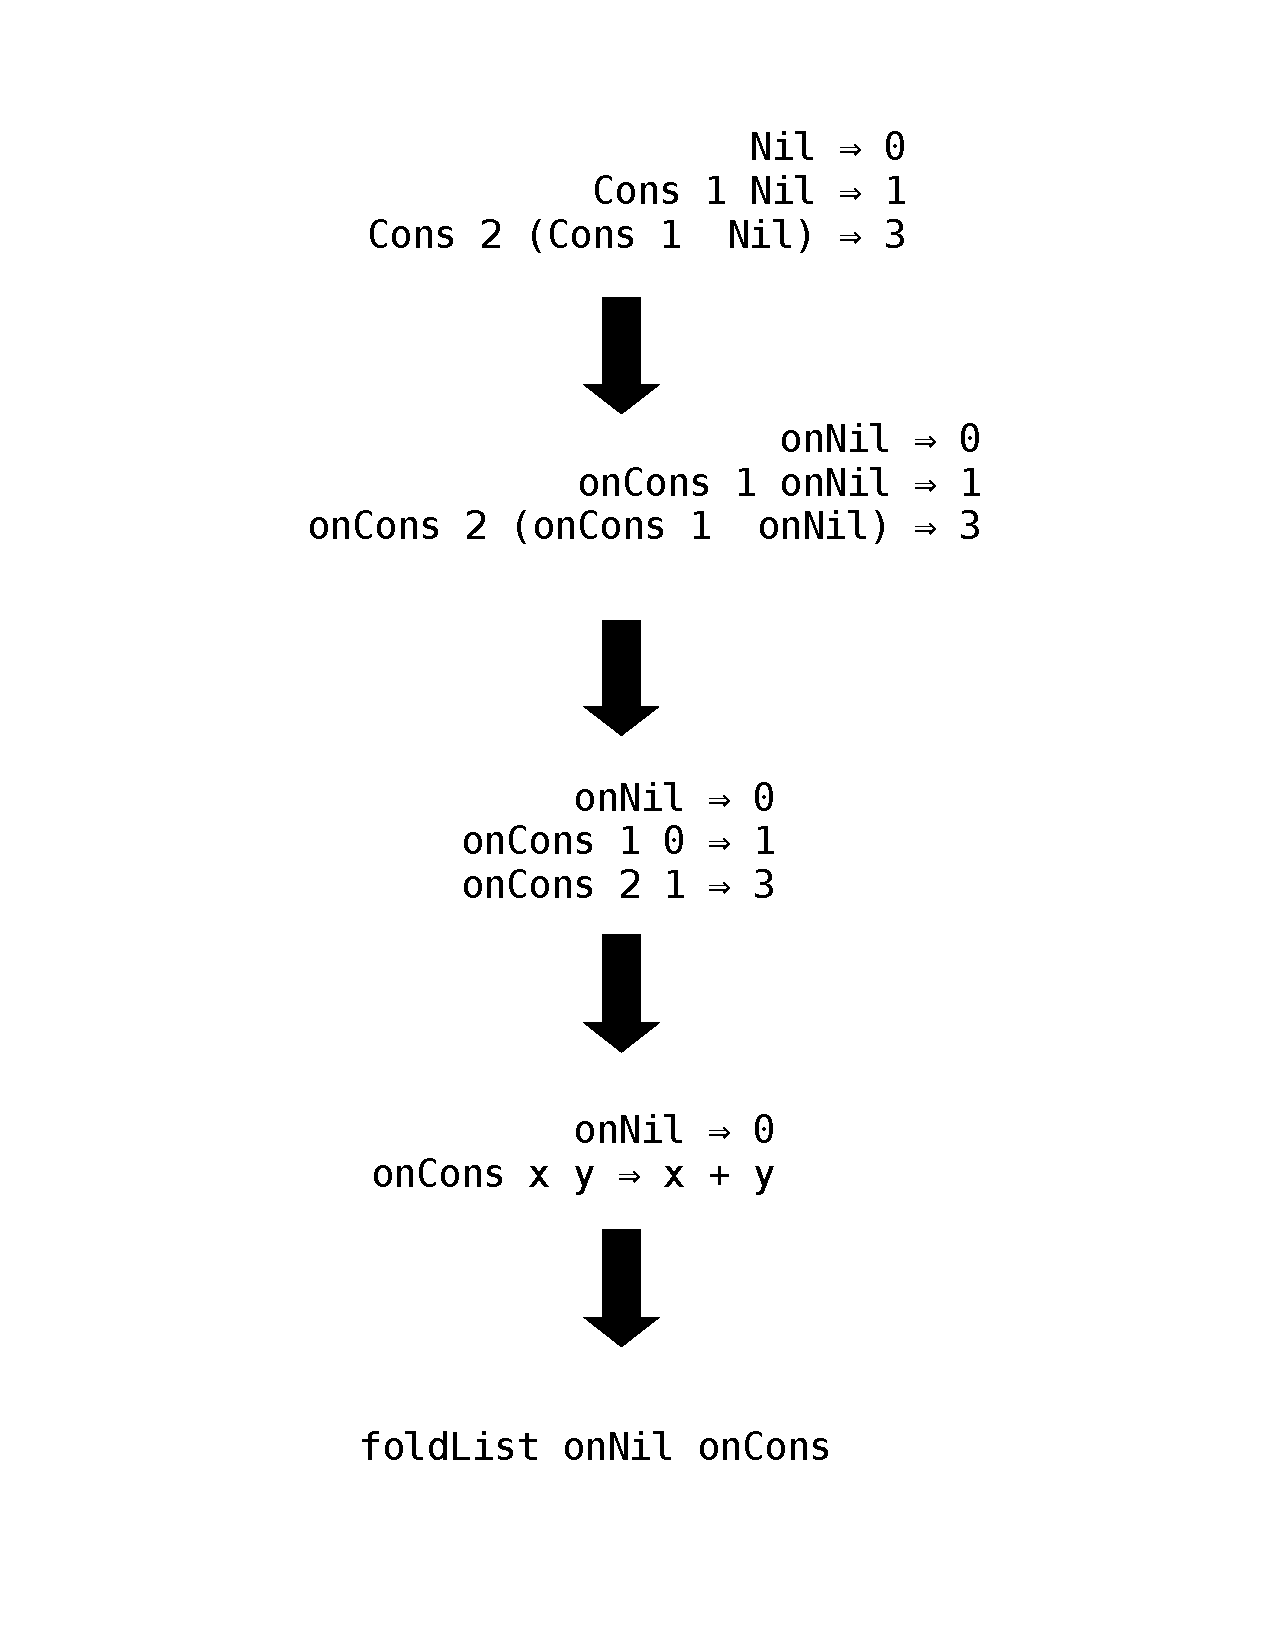
\includegraphics[width=0.4\textwidth]{Diagram.pdf}
\end{figure}


\section{Implementation}

We have implemented the Dan algorithm in Idris, a general-purpose, dependently-typed, purely-functional programming language with compile-time reflection capabilities(TODO: CITE). While we make heavy use of Idris' expressive type system to ensure the correctness of our implementation, we do not believe it required for a well-typed implementation of this algorithm. We also (TODO: CURRENTLY DO NOT) make use of Idris' ability to perform compile-time reflection in order to derive \texttt{Generic} implementations for types, and while languages without this feature may require more boilerplate, it is not impossible to perform.

<TODO: DOCUMENT USE OF IDRIS2-SOP>
<TODO: WHAT ELSE GOES HERE?>

\section{Evaluation}

To test our implementation, we extend a simple bottom-up enumerative synthesizer using Dan. As the underlying synthesizer is also language-polymorphic, we are able to generate a large set of interesting programs. In a simple calculator language, we're able to synthesize factorial and (TODO: CURRENTLY ONLY WITH A CONSTANT POWER) exponentiation. In a simple dynamically typed languages, we're able to synthesize tree-traversals and evaluators for simple languages. 

<TODO: COMPARE WITH OTHER SYSTEMS ONCE IMPLEMENTATION IS BETTER>

\section{Future Work}

<TODO: THIS SHOULD BE WRITTEN ONCE WORK IS DONE>

% Immediate next steps forwards for the Dan project would be expanding the implementation. Currently, it can only generate programs in dynamically typed programs - all terms and subterms must be instances of a single Object type, which is different for each language. This works, but limits the opportunities for pruning possible programs and makes expressing problems in the implementation language awkward. Another major improvement would be expressing new kinds of recursion other than \texttt{fold}, and defining multiple implementations of \texttt{fold} for different datatypes.

% It would also be helpful to further develop the connection between Dan and its category-theoretic notions. Currently, the only scheme provided is a catamorphism, but providing options such as a paramorphism or hyglomorphism would extend its synthesis abilities significantly.

% Lastly, Dan needs to be evaluated more thoroughly, both in isolation and compared to other tools, such as ESCHER and $\lambda^2$. Becoming competitive with these projects may require some performance engineering, as the current implementation was written primarily for ease of reading and experimentation.

% \begin{acks}
%     I would like to thank Nada Amin and William Byrd for their initial ideas for and implementation of this project. They have been a fantastic help both within 252R and without. I'd also like to thank Nada (again) and Tyler Holloway for teaching the class this semester. It's been incredibly engaging and has lead me to meet several interesting new people. I'd also like to thank the other members of the class for their great presentations, both of their work and their own, and comments about presented work, keeping the class interactive and inquisitive. I'd finally like to thank Dan Friedman, after whom the project is named, for his teaching style, which inspired the technique itself.
% \end{acks}

\section*{References}

<TODO: FIGURE OUT BIBTEX!!!>

% \begin{enumerate}
%   \item Peter-Michael Osera and Steve Zdancewic. 2015. Type and Example Directed Program Synthesis. SIGPLAN Not. 50, 6 (June 2015), 619–630. https://doi.org/10.1145/2813885.2738007
%   \item Albarghouthi, Aws and Gulwani, Sumit and Kincaid, Zachary. 2013. Recursive Program Synthesis. Proceedings of the 25th international conference on Computer Aided Verification. CAV'13. https://www.microsoft.com/en-us/research/publication/recursive-program-synthesis/
%   \item John K. Feser, Swarat Chaudhuri, and Isil Dillig. 2015. Synthesizing data structure transformations from input-output examples. SIGPLAN Not. 50, 6 (June 2015), 229–239. https://doi.org/10.1145/2813885.2737977
%   \item Jeremy Gibbons and Oege de Moor. 2003. The Fun of Programming. Palgrave. 41-60.
% \end{enumerate}

\end{document}

% LocalWords:  subproblems
